% -*- coding: utf-8 -*-
% !TEX program = xelatex

%\documentclass[11pt,a4paper]{article}
\documentclass[12pt,final]{article}

\usepackage[UTF8]{ctex}
\usepackage{amsmath,amsthm,amssymb}
\usepackage{mathrsfs}
\usepackage{graphicx}
\usepackage{subfig}
%\usepackage[english]{babel}
\usepackage{color,xcolor}
\usepackage{enumitem}
\usepackage{lipsum} % 用于生成示例文本
\usepackage{float}
\usepackage{pifont}
\usepackage{tabularx}
\usepackage{booktabs}
\usepackage{array}
\usepackage{multirow,multicol}
\usepackage{longtable}
\usepackage{makecell}
\usepackage{anyfontsize}
%\usepackage{microtype}
\usepackage{geometry}
\usepackage{relsize} % For smaller command
%\geometry{left=1.25in,right=1.25in,top=1in,bottom=1in}
\geometry{left=3cm,right=3cm,top=3cm,bottom=3cm}
\setlength{\headheight}{18pt}
\setlength{\headsep}{18pt}
\setlength{\footskip}{25pt}

%----- 设置超链接 -----
\usepackage{hyperref}
\hypersetup{
	colorlinks=true,
	linkcolor=black,
	citecolor=blue,
	filecolor=blue,
	urlcolor=blue
}

% 允许多行公式跨页显示
\allowdisplaybreaks

%----- 定义页眉-----
\makeatletter
\newcommand\@header{}
\newcommand\header[1]{\def\@header{#1}}
\makeatother

%----- 页眉页脚 -----
\usepackage{fancyhdr}
\makeatletter
\pagestyle{fancy}
\fancyhf{}
\fancyhead[C]{\small\kaishu\@header}
\fancyfoot[C]{\small\thepage}
\renewcommand{\headrulewidth}{0.5pt}
\makeatother

%----- 设置英文字体 -----
%\usepackage[no-math]{fontspec}
%\usepackage{newtxtext}  % New TX font for text
%\setmainfont{TeX Gyre Termes}  % Times New Roman 的开源复刻版本
%\setsansfont{TeX Gyre Heros}   % Helvetica 的开源复刻版本
%\setmonofont{TeX Gyre Cursor}  % Courier New 的开源复刻版本
%\setmainfont{Times New Roman}
%\setsansfont{Arial}
%\setmonofont{Courier New}

%----- 设置数学字体 -----
%\usepackage{newtxmath}
%\usepackage{mathptmx}

%----- 设置编号格式 -----
\numberwithin{equation}{section}
\numberwithin{figure}{section}
\numberwithin{table}{section}

%----- 重新设置图表公式 autoref -------
\renewcommand{\figureautorefname}{图}
\renewcommand{\tableautorefname}{表}
\renewcommand{\equationautorefname}{公式}

%----- 设置各种间距 -----
%\renewcommand{\baselinestretch}{1.35}
%\setlength{\parindent}{2em}
%\ziju{0.1}  % 控制中文字间距
%\setlength{\parskip}{3pt plus1pt minus1pt}

%----- 算法环境 -----
\usepackage{algorithm}
\usepackage{algpseudocode}
\floatname{algorithm}{算法}
\algrenewcommand\algorithmicrequire{\textbf{输入:}}
\algrenewcommand\algorithmicensure{\textbf{输出:}}

%----定义列表项的样式 -----
\usepackage{enumitem}
\setlist{nolistsep}

%-----设置图片的路径 -----
\graphicspath{{./figure/}{./figures/}}

%----- 使用 tabularx库并定义新的左右中格式 -----
\newcolumntype{L}{X}
\newcolumntype{C}{>{\centering \arraybackslash}X}
\newcolumntype{R}{>{\raggedleft \arraybackslash}X}
\newcolumntype{P}[1]{>{\centering \arraybackslash}p{#1}}

%----- 数学定理设置 -----
\theoremstyle{plain}
%\newtheorem{definition}{定义}[section]
%\newtheorem{proposition}{命题}[section]
%\newtheorem{lemma}{引理}[section]
%\newtheorem{theorem}{定理}[section]
%\newtheorem{example}{例}
%\newtheorem{corollary}{推论}[section]
%\newtheorem{remark}{注}[section]
\renewcommand{\proofname}{proof}
%\newtheorem{assumption}[theorem]{假设} % [theorem] 表示与定理共享编号

% 定义定理环境
\newtheorem{theorem}{Theorem}[section]   % [section] 表示按章节编号
\newtheorem{lemma}[theorem]{Lemma}      % [theorem] 表示与定理共享编号
\newtheorem{corollary}[theorem]{Corollary}  % [theorem] 表示与定理共享编号
\newtheorem{proposition}[theorem]{Proposition} % [theorem] 表示与定理共享编号
\newtheorem{assumption}[theorem]{Assumption} % [theorem] 表示与定理共享编号
% 定义定义环境
\theoremstyle{definition}
\newtheorem{definition}[theorem]{Definition}  % [theorem] 表示与定理共享编号
\newtheorem{example}[theorem]{Example}       % [theorem] 表示与定理共享编号
% 定义注释环境
\theoremstyle{remark}
\newtheorem{remark}[theorem]{Remark}      % [theorem] 表示与定理共享编号


\makeatletter
\renewenvironment{proof}[1][\proofname]{\par
	\pushQED{\qed}%
	\normalfont \topsep6\p@\@plus6\p@\relax
	\trivlist\item[\hskip\labelsep
	\bfseries #1\@addpunct{\,:\,}]\ignorespaces
}{%
	\popQED\endtrivlist\@endpefalse
}
\makeatother

%----- 参考文献格式 -----
%\bibliographystyle{plain} % abbrv, unsrt, siam
\bibliographystyle{thuthesis-numeric}
%\bibliographystyle{thuthesis-author-year}

%----- 参考文献引用格式 -----
\usepackage[numbers,sort&compress]{natbib}
%\usepackage[numbers,super,square,sort&compress]{natbib}
\def\bibfont{\small}  % 修改参考文献字体
\setlength{\bibsep}{7pt plus 3pt minus 3pt}  % 调整参考文献间距

%----- 微分符号 -----
\newcommand{\dif}{\mathop{}\!\mathrm{d}}

%----- 定义新命令 -----
\newcommand{\CC}{\ensuremath{\mathbb{C}}}
\newcommand{\RR}{\ensuremath{\mathbb{R}}}
\newcommand{\abs}[1]{\lvert#1\rvert}
\newcommand{\norm}[1]{\lVert#1\rVert}
\newcommand{\dx}[1][x]{\mathop{}\!\mathrm{d}#1}
\newcommand{\ii}{\mathrm{i}\mkern1mu} % imaginary
\newcommand{\refe}[2]{(\ref{#1})--(\ref{#2})}
\newcommand{\A}{\mathcal{A}}
\newcommand{\bA}{\boldsymbol{A}}
\newcommand{\red}[1]{\textcolor{red}{#1}}

%----- 论文信息 -----
\header{毕业论文}

\title{毕业论文}
\author{左如春}
\date{\today}


\begin{document}
	
	\maketitle
	
	\begin{abstract}
		研究Euler-Maruyama (EM)数值逼近一类经过Lamperti变换后,漂移系数线性增长、扩散系数是常数的时变随机微分方程.证明了EM的强收敛性与逆从属的稳定指数之间的关系,并讨论收敛速度.并通过数值模拟验证了理论结果.
		
		\medskip
		\noindent\textbf{关键词:} 时间变换;等距离散;收敛阶;逆从属.
	\end{abstract}
	
	%%%%%%%%%%%%%%%%%%%%%%%%%%%%%%%%%%%%%%%%%%%%%
	
	%\tableofcontents
	
	%%%%%%%%%%%%%%%%% 正文开始 %%%%%%%%%%%%%%%%%%%
	
	%%%%%%%%%%%%%%%%% 引言 %%%%%%%%%%%%%%%%%%%%%%
	
	\section{Introduction}
	
	受到\cite{Alfonsi2013602}的启发,本文的目的是推导出一个有效的数值逼近具有全局Lipschitz的漂移系数和扩散项系数的一维随机微分方程.主要思想是使用Lamperti变换将原始的时变SDE转化成带有加性噪声的时变SDE,见\cite{iacus2008simulation},通过EM对变换后的时变SDE进行逼近,再将其变换成原始时变SDE的逼近格式.
	
	对于时间变换的随机微分方程,现在已经有了很多的数值逼近格式.在\cite{jum2014strong}中证明了对于漂移项和扩散项都满足全局Lipschitz时,可以采用对偶原则,将时间变换随机微分方程转换成一般随机微分方程,通过对一般随机微分方程使用EM数值格式进行逼近,进而得到时间变换随机微分方程的强收敛阶.在\cite{deng2020semi}中将这一思想运用在漂移项满足非全局Lipschitz条件时,使用半隐式EM得到强收敛阶,并研究了其稳定性.这解决了一大类可以对偶化的时间变换微分方程的数值格式收敛性问题.在\cite{jin2019strong},对于不能使用对偶原则的时间变换随机微分方程,采用一种非等距的离散格式,并得到强收敛阶.纵观以往的时间变换的随机微分方程的数值格式,大多采用的是非等距离散.而在这篇文章中,我们将使用等距离散来研究随机微分方程:
	\begin{equation}\label{basic SDE}
		dX(s)=f(X(s))dE(s)+\sigma dB(E(s))
	\end{equation}
	
	\section{Preliminaries}
	
	在这篇文章中,$(\Omega,\mathcal{F},\mathbb{P})$ 表示完备概率空间 , $D=(D_t)_{t\geq0}$ 表示具有Laplace指数$\psi$,从0开始的从属,其中$\psi$的被杀率是0且具有Lévy测度$\nu;$ 即$D$是具有开始于0的càdlàg路径的一维非减Lévy过程,其Laplace变换是:
	$$\mathbb{E}[e^{-sD_t}]=e^{-t\psi(s)},\quad\text{其中}\quad\psi(s)=\int\limits_0^\infty(1-e^{-sy})\:\nu(\text{d}y),\quad s>0,$$
	并且 $\int_0^\infty(y\wedge1)\nu(dy) < \infty$,
	我们考虑Lévy测度$\nu$是无穷的情况,即$\nu ( 0, \infty ) = \infty$,这意味着复合泊松从属不在我们的考虑范围中.令 $E=(E_t)_{t\geq0}$是$D$的逆,即:
	$$E_t:=\inf\{u>0;D_u>t\},\:t\geq0.$$
	我们称$E$是逆从属,注意$E$是连续且非递减的.一般我们假设$B(t)$ 和 $D(t)$ 是相互独立的. 随机过程$B(E(t))$被称作时间变换的布朗运动.我们注意到$D(t)$的跳跃部分和$E(t)$的平坦部分相互对应的.又由于$E(t)$的平坦部分,导致$B(E(t))$在这一部分也是平坦的,因此$B(E(t))$可以被理解成是一种次扩散.
	
	令 $S=(l,r)$, 其中 $-\infty\leq l<r\leq\infty$,函数 $a,b$是$S\to S$ 的连续可微函数. 考虑下面的SDE:
	$$dy(t)=a(y(t))dE(t)+b(y(t))dB(E(t)),\quad t\geq0,\quad y(0)\in S$$
	并且假设它在S中有唯一强解,即
	$$\mathbb{P}(y(t)\in S,\:t\geq0)=1.$$
	如果 $b(x)>0$ 对所有的 $x\in S$都成立, 那么我们可以使用Lamperti变换
	$$F(x)=\lambda\int^x\frac1{b(y)}dy$$
	对于某些$\lambda>0.$并且$F^{-1}:F(S)\to S$ 是被良好定义的, 令$x(t)=F(y(t))$利用\cite{umarov2018beyond}中的时间变换Itô公式可以得到:
	$$dx(t)=f(x(t))dE(t) + \lambda dB(E(t)) \quad t\geq0,\quad x(0)\in F(S)$$
	其中
	$$f(x)=\lambda\left(\frac{a(F^{-1}(x))}{b(F^{-1}(x))}-\frac12b^{\prime}(F^{-1}(x))\right),\quad x\in F(S),$$
	$F(D)=(F(l),F(r)).$ 这种变换可以将扩散项的非线性项转换到漂移项中
	\section{Some Assumptions and Lemmas}
	\begin{assumption}\label{assum1}
		令$-\infty\leq\alpha<\beta\leq\infty$,并且假设时间变换的SDE(\ref{basic SDE})在$(\alpha,\beta)\subseteq\mathbb{R}$有唯一强解,即:$$\mathbb{P}(x(t)\in(\alpha,\beta), t\geq0)=1.$$
	\end{assumption}
	\cite{KaratzasShreveBM}中的Feller test可以\textcolor{red}{直接推广}到时间变换SDE中,因此Assumption\ref{assum1}等价于:
	\begin{equation}\label{v(x)}
		\lim\limits_{x\to\alpha_+}v(x)=\infty,\quad\lim\limits_{x\to\beta_-}v(x)=\infty
	\end{equation}
	其中
	$$v(x)=\frac{2}{\sigma^2}\int\limits_{x_0}^x\int\limits_{x_0}^{\zeta_2}\frac{p'(\zeta_2)}{p'(\zeta_1)}d\zeta_1d\zeta_2$$
	尺度函数$p(x)$是:
	$$p(x)=\int\limits_{x_0}^x\exp\left(-2\int\limits_{x_0}^\xi\frac{f(u)}{\sigma^2}du\right)d\xi,\quad x\in(\alpha,\beta).$$
	于是:$$v(x)=\frac{2}{\sigma^2}\int\limits_{x_0}^x\int\limits_{x_0}^{\zeta_2}\exp\left(-2\int\limits_{\zeta_1}^{\zeta_2}\frac{f(u)}{\sigma^2} du\right)d\zeta_1d\zeta_2.$$
	\textcolor{red}{可以验证}对于有限的$\alpha$和$\beta$,\eqref{v(x)}等价于:$$\lim\limits_{x\to\alpha_+}\sup f(x)=\infty,\quad\lim\limits_{x\to\beta_-}\inf f(x)=-\infty.$$
	\begin{assumption}\label{assum2}
		令$c\in[-\infty,+\infty),I=(c,+\infty),\operatorname{}d\in I$是区间中任意的一点. 假设漂移项系数$f$满足下述单调性 :
		\begin{equation}
			f:I\to\mathbb{R}  , 使得 \exists\kappa\in\mathbb{R},\forall x,x^\prime\in I,x\leq x^\prime,f(x^\prime)-f(x)\leq\kappa(x^\prime-x).
		\end{equation}
	\end{assumption}
	\begin{assumption}\label{assum3}
		令$T>0$,假设漂移项系数$f$是二阶连续可微的并且满足:
		\begin{equation}
			\sup\limits_{t\in[0,T]}\mathbb{E}\left|f'(x(t))\right|^2+
			\sup\limits_{t\in[0,T]}\mathbb{E}\left|f(x(t))'f(x(t))+
			\frac{\sigma^2}2f''(x(t))\right|<\infty.
		\end{equation}
	\end{assumption}
	时间变换SDE(\ref{basic SDE})的强解存在唯一性可以由\cite{kobayashi2011stochastic}中的定理4.1直接得到
	\begin{assumption}
		一些正解的假设,Feller Test
	\end{assumption}
	从\cite{umarov2018beyond}可以得到下面的时间变换的$Ito$公式
	\begin{lemma}\label{ito}
		令 Z 是一维标准的布朗运动. 令 $D$ 和 $E$ $be$ $a$ 满足 $[ [ D\longmapsto E] ]$ $or$ $[ [ U\longleftrightarrow E] ] .$ X是由下述SDE定义的随机过程
		$$X_t:=\int_0^tA_sds+\int_0^tF_sdE_s+\int_0^tG_sdZ_{E_s}$$
		其中 $A\in$ $L( t, \mathcal{F} _{E_t})$, $F\in$ $L( E_t, \mathcal{F} _{E_t})$, 以及 $G\in$ $L( Z_{E_t}, \mathcal{F} _{E_t}) .$ 如果 $f\in$ $C^2( \mathbb{R} )$, 那么
		$f( X) \textit{ 是 ( F}_{E_t}) - $半鞅, 对于所有的t $\ge$ 0,都有
		$$\begin{aligned}
			&f(X_{t})-f(0)=\int_{0}^{t}f^{\prime}(X_{s})A_{s}ds+\int_{0}^{E_{t}}f^{\prime}\left(X_{D(s-)}\right)F_{D(s-)}ds\\
			&+\int_{0}^{E_{t}}f^{\prime}\big(X_{D(s-)}\big)G_{D(s-)}dB_{s}+\frac{1}{2}\int_{0}^{E_{t}}f^{\prime\prime}\big(X_{D(s-)}\big)\big\{G_{D(s-)}\big\}^{2}ds.
		\end{aligned}$$
	\end{lemma}
	% 使用BEM时,需要使用这个定理,并将\Delta t修改成\Delta E
	\begin{lemma}\label{lemma:1}
		令$\Delta t > 0,g_n,\lambda _n \in \mathbb{R},\eta > 0$,再假设$1-\eta \Delta t > 0$,$1 + \lambda _n > 0,n \in \mathbb{N}$,那么如果
		\begin{equation*}
			a_{n+1} \leq a_n(1+\lambda _n)+\eta a_{n+1}\Delta t +g_{n+1}
		\end{equation*}
		则下面的不等式成立:
		\begin{equation}
			a_n \leq \frac{1}{(1-\eta\Delta t)^n}\sum\limits_{j=0}^{n-1}(1-\eta\Delta t)^jg_{j+1}\prod\limits_{l=j+1}^{n-1}(1+\lambda _l)
		\end{equation}
	\end{lemma}
	下面的引理对于证明定理起着关键性的作用.
	\begin{lemma}\label{lemma:2}
		对于任意给定的$0 = t_0 < ih < t_1 < t_2 < \ldots <t_n <(i+1)h$,都有:
		\begin{equation}
			\mathbb{E}\left[\int_{ih}^{(i+1)h}
			\int_{ih}^{t_n} \ldots \int_{ih}^{t_2} 1 dE_{t_1} \ldots dE_{t_{n-1}}dE_{t_n}\right] \le Ch^{1+(n-1)\beta}
		\end{equation}
		,其中C是与$h$无关的常数.
	\end{lemma}
	
	
	\begin{proof}    
		在\cite{daley2003introduction}和\cite{magdziarz2009stochastic}中可以直接得到,如果$0 = t_0 < t_1 < t_2 < \ldots <t_n$,那么:
		\begin{equation*}
			\mathbb{E}[\mathrm dE_\alpha(t_n)\ldots\mathrm dE_\alpha(t_1)]=\prod_{i=1}^nu'(t_i-t_{i-1})\mathrm dt_i.
		\end{equation*}
		其中$u(t)=\mathbb{E}[E_\alpha(t)]=\frac{t^\alpha}{\Gamma(1+\alpha)}$,因此:
		\begin{align*}
			I &= \mathbb{E}\left[\int_{ih}^{(i+1)h}
			\int_{ih}^{t_n}\int_{ih}^{t_{n-1}} \ldots \int_{ih}^{t_{2}} 1 dE_{t_1} \ldots dE_{t_{n-2}}dE_{t_{n-1}}dE_{t_n}\right] \\
			& = \int_{ih}^{(i+1)h}\int_{ih}^{t_n}\int_{ih}^{t_{n-1}}
			\ldots \int_{ih}^{t_{2}} 1 \mathbb{E}\left[dE_{t_1} \ldots dE_{t_{n-2}}dE_{t_{n-1}}dE_{t_n}\right] \\
			& = \frac{\alpha^n}{\Gamma^n(\alpha+1)}
			\int_{ih}^{(i+1)h}\int_{ih}^{t_n}\int_{ih}^{t_{n-1}} \ldots \int_{ih}^{t_{2}} \prod_{i=1}^{i=n}(t_i-t_{i-1})^{\alpha -1} dt_1 \ldots dt_{n-1}dt_n
		\end{align*}
		
		下面单独考虑积分项:
		\begin{align*}
			I_{1}=\int_{ih}^{t_{2}} (t_{2}-t_1)^{\alpha -1} t_1^{\alpha - 1} dt_1 \\
		\end{align*}
		做如下变换,令$t_{1} = ih + s_{1}h$,同时$t_2 = ih + s_2h ,$,其中$h$是步长,因此$s_1,s_{2} \in [0,1]$,注意由于我们不考虑时间在原点处,因此这里的$i=\frac{T}{h}$,这里的$T$是一个时间范围,于是
		\begin{align*}
			I_1 &= \int_{0}^{s_{2}} (s_{2}-s_{1})^{\alpha -1}h^{\alpha -1} (ih + s_1h)^{\alpha - 1}h ds_1 \\
			&= h^{\alpha}\int_{0}^{s_{2}} (s_{2}-s_{1})^{\alpha -1} (ih + s_1h)^{\alpha - 1} ds_1
		\end{align*}
		由于$(ih + s_1h)^{\alpha - 1}$关于$s_1$在$[0,1]$是单调递减的,并且积分$I_n$中,被积函数和积分区域都是正的,因此
		\begin{align*}
			I_1 &\le h^{\alpha}\int_{0}^{s_{2}} (s_{2}-s_{1})^{\alpha -1} (ih)^{\alpha - 1} ds_1 \\
			&=  T^{\alpha - 1}h^{\alpha}\int_{0}^{s_{2}} (s_{2}-s_{1})^{\alpha -1} ds_1
		\end{align*}
		令$w_1=s_{2}-s_{1}$,于是
		\begin{equation*}
			I_1\le T^{\alpha - 1}h^{\alpha}\int_{0}^{s_{2}} (s_{2}-s_{1})^{\alpha -1} ds_1
			=  T^{\alpha - 1}h^{\alpha}\int_{0}^{s_{n2}} w_1^{\alpha -1} dw_1
			=  \frac{T^{\alpha - 1}s_{2}^\alpha}{\alpha}h^{\alpha}
		\end{equation*}
		因此:
		\begin{equation*}
			I \le Ch^\alpha
			\int_{ih}^{(i+1)h}\int_{ih}^{t_n}\int_{ih}^{t_{n-1}} \ldots \int_{ih}^{t_{3}} 
			\prod_{i=3}^{n}(t_i-t_{i-1})^{\alpha -1} dt_{2} \ldots dt_{n-1}dt_n
		\end{equation*}
		
		同理,分析如下积分:
		\begin{equation*}
			I_{2} = \int_{ih}^{t_{3}}(t_{3}-t_{2})^{\alpha -1}
			dt_{2} \le Ch^\alpha 
		\end{equation*}
		
		因此:
		\begin{equation*}
			I \le Ch^{2\alpha}
			\int_{ih}^{(i+1)h}\int_{ih}^{t_n}\int_{ih}^{t_{n-1}} \ldots \int_{ih}^{t_{4}} 
			\prod_{i=4}^{n}(t_i-t_{i-1})^{\alpha -1} dt_{3} \ldots dt_{n-1}dt_n
		\end{equation*}
		如此进行迭代,我们得到:
		\begin{equation*}
			I \le Ch^{(n-1)\alpha}\int_{ih}^{(i+1)h} 1 dt_1 \le Ch^{1+(n-1)\alpha}
		\end{equation*}
		因此,得到收敛阶为$1+(n-1)\alpha$
	\end{proof}
	
	\section{Main results}
	
	对于随机微分方程\eqref{basic SDE},它的BEM数值格式是:
	\begin{equation}\label{eq:1}
		X_{t_{i+1}}^{\delta}=X_{t_i}^{\delta}+f(x_{t_{i+1}}^{\delta})\Delta E_{i}+\sigma\Delta B_{E_{i}},\quad i=0,1,2,\ldots,\qquad X_0^\delta=X(0)
	\end{equation}
	其中$\Delta E_{i}=E(t_{i+1})-E(t_i)$以及$\Delta B_{E_{i}}=B_{E{(t_{i+1})}}-B_{E({t_i})}$.
	\begin{theorem}\label{main th}
		对于任意的$\epsilon>0$,令$\epsilon < T1 < T2$,在假设\ref{assum1},\ref{assum2}和\ref{assum3}的条件下,存在常数C,使得下面的不等式成立:
		$$\mathbb{E}[|X({t_i})-X_{t_i}^{\delta}|]\le C\Delta t^\alpha,\quad i=\lceil T1/\Delta t \rceil,\lceil T1/\Delta t \rceil+1 \ldots \lceil T2/\Delta t \rceil$$
	\end{theorem}
	\begin{proof}
		考虑SDE(\ref{basic SDE})在$[t_i,t_{i+1})$的积分:
		\begin{align}
			\int_{t_i}^{t_{i+1}}dX(s)=\int_{t_i}^{t_{i+1}}f(X(s))dE(s)+\int_{t_i}^{t_{i+1}}\sigma dB(E(s))
		\end{align}
		等价于
		\begin{align}
			\int_{t_i}^{t_{i+1}}dX(s))=\int_{E_{t_i}}^{E_{t_{i+1}}}f(X(D(s-)))ds+\int_{E_{t_i}}^{E_{t_{i+1}}}\sigma dB(s)
		\end{align}
		针对于漂移项$f(X(D-(s-)))$,下面等式恒成立:
		\begin{align}\label{eq:ito}
			\int_{E(t_i)}^{E(t_{i+1})} f(X(D(t_{i+1}-)))) - f(X(D(t-))) dt = \int_{E(t_i)}^{E(t_{i+1})} \int^{D(t_{i+1}-)}_{D(t_-)} df(X(s)) dt
		\end{align}
		对于$df(X(s))$,由Lemma\ref{ito}的时间变换$ito$公式:
		\begin{align*}
			\begin{gathered}
				f(X_{t})-f(0)=\int_{0}^{E_{t}}f(X(D(s-)))f^{\prime}\left(X_{D(s-)}\right)+\frac{\sigma^{2}}{2}f^{\prime\prime}\big(X_{D(s-)}\big)ds \\
				+\int_{0}^{E_{t}}\sigma f^{\prime}\big(X_{D(s-)}\big)dB_{s}
			\end{gathered}
		\end{align*}
		于是\eqref{eq:ito}变成
		\begin{equation}\label{eq:ito1}
			\begin{aligned}
				&\quad\int_{E(t_i)}^{E(t_{i+1})} f(X(D(t_{i+1}-))) - f(X(D(t-))) dt \\
				&= \int_{E(t_i)}^{E(t_{i+1})} \int_{t}^{t_{i+1}} \left( f(X(D(s))) f^{\prime}(X(D(s))) + \frac{1}{2} \sigma^2 f^{\prime\prime}(X(D(s))) \right) ds \, dt\\
				&\quad + \int_{E(t_i)}^{E(t_{i+1})} \int_{t}^{t_{i+1}} \sigma f^{\prime}(X(D(s))) \, dB(s) \, dt .
			\end{aligned}
		\end{equation}
		由\eqref{basic SDE}与\eqref{eq:ito1},以及\cite[Theorem 3.1]{kobayashi2011stochastic}可以得到
		\begin{align*}
			X(t_{i+1}) 
			&= X(t_i) + \int_{E(t_i)}^{E(t_{i+1})} f(X({D(t_{i+1})})) \, dt + \int_{t_i}^{t_{i+1}} \sigma \, dB(E(t)) \\
			&\quad + \int_{E(t_i)}^{E(t_{i+1})} \int_{t}^{t_{i+1}}\left( f(X(D(s))) f^{\prime}(X(D(s))) + \frac{1}{2} \sigma^2 f^{\prime\prime}(X(D(s))) \right) ds \, dt \\
			&\quad + \int_{E(t_i)}^{E(t_{i+1})} \int_{t}^{t_{i+1}}\sigma f^{\prime}(X(D(s)))) \, dB(s) \, dt \\
			&= X(t_i) + \int_{t_i}^{t_{i+1}} f(X({t_i)}) \, dE(t) + \int_{t_i}^{t_{i+1}} \sigma \, dB(E(t)) \\
			&\quad + \int_{t_i}^{t_{i+1}} \int_{E(t)}^{E(t_{i+1})} \left( f(X(D(s))) f^{\prime}(X(D(s))) + \frac{1}{2} \sigma^2 f^{\prime\prime}(X(D(s))) \right) ds \, dE(t) \\
			&\quad + \int_{t_i}^{t_{i+1}} \int_{E(t)}^{E(t_{i+1})}\sigma f^{\prime}(X(D(s))) \, dB(s) \, dE(t)\\
			&= X(t_i) + \int_{t_i}^{t_{i+1}} f(X({t_i})) \, dE(t) + \int_{t_i}^{t_{i+1}} \sigma \, dB(E(t)) \\
			&\quad + \int_{t_i}^{t_{i+1}} \int_{t}^{t_{i+1}} \left( f(X(s)) f^{\prime}(X(s)) + \frac{1}{2} \sigma^2 f^{\prime\prime}(X(s)) \right) dE(s) \, dE(t) \\
			&\quad + \int_{t_i}^{t_{i+1}} \int_{t}^{t_{i+1}}\sigma f^{\prime}(X(s)) \, dB(E(s)) \, dE(t)
		\end{align*}
		因此
		\begin{align}\label{eq:2}
			X(t_{i+1})
			&= X(t_i) + \int_{t_i}^{t_{i+1}} f(X({t_{i+1})}) \, dE(t) + \int_{t_i}^{t_{i+1}} \sigma \, dB(E(t)) + R_i
		\end{align}
		令$R_i = -\int_{t_i}^{t_{i+1}} \int_{t}^{t_{i+1}} \left( f(X(s)) f^{\prime}(X(s)) + \frac{1}{2} \sigma^2 f^{\prime\prime}(X(s)) \right) dE(s) \, dE(t)-\int_{t_i}^{t_{i+1}} \int_{t}^{t_{i+1}} \sigma f^{\prime}(X(s)) \, dB(E(s)) \, dE(t).$\\
		将$R_i$分解成$R_s = R_s^{(1)} + R_s^{(2)}$,其中:
		\begin{align*}
			& R_s^{(1)} = -\int_{t_i}^{t_{i+1}} \int_{t}^{t_{i+1}} \left( f(X(s)) f^{\prime}(X(s)) + \frac{1}{2} \sigma^2 f^{\prime\prime}(X(s)) \right) dE(s) \, dE(t).\\
			& R_s^{(2)} = -\int_{t_i}^{t_{i+1}} \int_{t}^{t_{i+1}} \sigma f^{\prime}(X(s)) \, dB(E(s)) \, dE(t)  
		\end{align*}
		和离散格式相减,即(\ref{eq:2})-\eqref{eq:1}得到:
		\begin{equation}
			X({t_{i+1}})-X_{t_{i+1}}^{\delta}=X({t_i})-X_{t_i}^{\delta}+(f{(x({t_{i+1}}))}-f{(x^\delta_{t_{i+1}})})\Delta E_{i}+R_{i}
		\end{equation}
		令$e_i = X({t_i})-X_{t_i}^{\delta}$
		由假设\ref{assum2}得到:
		\begin{equation}
			(1-K_1\Delta E_s)e_{s+1}\leq e_{s}+R_{s},\quad\text{其中}s=\lceil T1/\Delta t \rceil,\lceil T1/\Delta t \rceil+1 \ldots \lceil T2/\Delta t \rceil
		\end{equation}
		定义$\gamma_l = 1-K_1\Delta E_l$,$N_1 = \lceil T1/\Delta t \rceil$以及$N_2 = \lceil T2/\Delta t \rceil$,由于始终存在常数C,使得$\Delta E_l < C\Delta t$,从而可以得到
		$$\prod\limits_{l=N_1}^{N_2}\gamma_l^{-1} < \frac{1}{(1-C\Delta t)^{N_2-N_1}} < \infty.$$
		由Lemma\ref{lemma:1},我们可以得到
		$$e_{N_2} \leq \sum\limits_{j=N_1}^{N_2}R_{j}\prod\limits_{l=j}^{N_2}\gamma_l^{-1} \le C \sum\limits_{j=N_1}^{N_2}R_{j}$$
		于是
		$$\mathbb{E}  |e_{N_2}| \leq C\mathbb{E}|\sum\limits_{j=N_1}^{N_2}R_{j}^{(1)} | + C\mathbb{E}|\sum\limits_{j=N_1}^{N_2}R_{j}^{(2)} |$$.
		
		下面先考虑第一项,由Lemma\ref{lemma:2}和Assumption\ref{assum3},可以得到
		\begin{equation}
			\mathbb{E} |R_j^{(1)}| \le C\mathbb{E} \left[ \int_{t_i}^{t_{i+1}}\int_{t_i}^{t}1dEsdEt \right] \le C\Delta t^{1+\alpha}
		\end{equation}
		于是
		\begin{equation}
			\mathbb{E}|\sum\limits_{j=N_1}^{N_2}R_{j}^{(1)}\prod\limits_{l=j}^{N_2}\gamma_l|\leq C\sum\limits_{N_1}^{N_2}\mathbb{E}|R_{j}^{(1)}| \leq
			C\sum\limits_{j=N_1}^{N_2}\Delta t^{1+\alpha} \le C\Delta t^\alpha
		\end{equation}
		
		下面考虑第二项,因为$\mathbb{E}\left[ R_{k}^{(2)}|\mathcal{F}_{k\Delta t} \right] = \mathbb{E}_D\mathbb{E}_B\left[ \int_{t_i}^{t_{i+1}} \int_{t_i}^{t} \sigma f^{\prime}(X(s)) \, dB(E(s)) \, dE(t) \right]=\mathbb{E}_D\left[ \int_{t_i}^{t_{i+1}} \mathbb{E}_B\int_{t_i}^{t} \sigma f^{\prime}(X(s)) \, dB(E(s)) \, dE(t) \right]= 0$,因此
		\begin{align*}
			\sum_{j=N_1}^{N_2}R_{j}^{(2)} 
		\end{align*}
		是鞅
		
		下面考虑第二项$\mathbb{E}|\sum\limits_{j=N_1}^{N_2}R_{j+1}^{(2)}|$,在此之前通过BDG不等式和Lemma\ref{lemma:2}可以得到下面的不等式:
		\begin{equation}
			\mathbb{E}[dB_EdE]^2=\mathbb{E}[(dB_E)^2(dE)^2]=\mathbb{E}_D[(dE)^2\mathbb{E}_B(dB_E)^2]\leq
			C\mathbb{E}_{D}[dE]^3\leq C\Delta t ^{1+2\alpha}
		\end{equation}
		接下来使用BDG不等式和Cauchy-Schwarz不等式,可以得到:
		\begin{equation*}
			\mathbb{E}\left|\sum_{j=N_1}^{N_2}R_{j}^{(2)}\right|  \le C\mathbb{E} \left|\sum_{j=N_1}^{N_2}(R_{j}^{(2)})^2\right|^{\frac{1}{2}} \le C\sqrt{\sum_{j=N_1}^{N_2}\mathbb{E}(R_{j}^{(2)})^2}
			\le C\sqrt{\sum_{j=N_1}^{N_2}\Delta t^{1+2\alpha}} \le C\Delta t^{\alpha}
		\end{equation*}
		
		%\textcolor{red}{(2)}由于$\mathbb{E}|f'(X(s))|^2 < \infty$,因此对于$f'(X(s))$而言,在每个区间$[t_i,t_{i+1}]$都存在一个$S_i$使得$\max_{t_{i}<t<t_{i+1}}f{(X_t)}=f{(X{(S_{i})})}$,并且存在一个$T_i \in [t_i,t_{i+1}]$使得$\max_{t_{i}<t<t_{i+1}}B(E(t))=B(E(T_i))$,因此:
		%\begin{equation*}
		%	\mathbb{E}\left|\sum_{j=\lceil T1/\Delta t \rceil}^{n}R_{j}^{(2)}\right|  =
		%	\mathbb{E} \left| \sum_{j=\lceil T1/\Delta t \rceil}^{n}\int_{t_i}^{t_{i+1}} \int_{t_i}^{t} \sigma f^{\prime}(X(s)) \, dB(E(s)) \, dE(t)   \right| \le \mathbb{E} \left| \sum_{j=\lceil T1/\Delta t \rceil}^{n}\int_{t_i}^{t_{i+1}} \int_{t_i}^{T_i} \sigma f^{\prime}(X(S_i)) \, dB(E(s)) \, dE(t)   \right|
		%\end{equation*}
		%接下来可以直接使用BDG不等式,可以得到:
		%\begin{equation*}
		%	\mathbb{E}_D\mathbb{E}_B \left| \sum_{j=\lceil T1/\Delta t \rceil}^{n} \int_{t_i}^{T_i} \sigma f^{\prime}(X(S_i)) \Delta E_i \, dB(E(s))   \right| \le C\mathbb{E}_D \left| \sum_{j=\lceil T1/\Delta t \rceil}^{n} \int_{t_i}^{T_i} (\Delta E_i)^2 \, dE(s)   \right|^{\frac{1}{2}}
		%\end{equation*}
		%下面由Cauchy-Schwarz不等式可以得到:
		%\begin{equation*}
		%	\mathbb{E}_D \left| \sum_{j=\lceil T1/\Delta t \rceil}^{n} \int_{t_i}^{T_i} (\Delta E_i)^2 \, dE(s)   \right|^{\frac{1}{2}} \le C\left|\mathbb{E}_D  \sum_{j=\lceil T1/\Delta t \rceil}^{n} \int_{t_i}^{T_i} (\Delta E_i)^2 \, dE(s)   \right|^{\frac{1}{2}} \le  C\left | \sum_{j=\lceil T1/\Delta t \rceil}^{n}\mathbb{E}_D(\Delta E_i)^3 \right|^{\frac{1}{2}}\le C\left | \sum_{j=\lceil T1/\Delta t \rceil}^{n}\Delta t^{1+2\alpha} \right|^{\frac{1}{2}} \le C \Delta t^{\alpha}
		%\end{equation*}
		
		综上所述,
		\begin{equation*}
			\mathbb{E} [e_n] \leq C\Delta t^\alpha
		\end{equation*}
	\end{proof}
	tips:We have also proved that $\mathbb{E} [\Delta E \Delta B_E ] \le C\Delta t ^{1+\frac{\alpha}{2}}$,however it seems that it's nothing help here.
	\section{Numerical examples}
	通过下述方法得到$D_\alpha(t)$的数值模拟格式:\\
	\begin{align*}
		&D_{\alpha}(0)=0,\\
		&D_{\alpha}(\delta n)=D_{\alpha}(\delta(n-1))+\delta^{1/\alpha}\xi_{n}
	\end{align*}
	其中$n=1,2,3 \ldots$并且$\xi_n$是独立同分布的完全偏斜的$\alpha$稳定随机变量,$\xi_n$的实现过程如下:
	\begin{align*}
		\xi_n=\frac{\sin(\alpha(V+c_1))}{\left(\cos(V)\right)^{1/\alpha}}\Big(\frac{\cos(V-\alpha(V+c_1))}{W}\Big)^{(1-\alpha)/\alpha}
	\end{align*}
	其中$c_1 = \frac{\pi}{2}$,随机变量$V$是$(-\frac{\pi}{2},\frac{\pi}{2})$上的均匀分布,$W$是均值为$1$的指数分布.
	\subsection{Examples}
	在这一节中,我们将主要结论应用到实际例子中.
	\subsubsection{CIR Process With Time-Changed Brownian Motion}
	回忆时间变换的CIR过程
	$$dy(t)=\kappa(\theta-y(t))dE(t)+\sigma\sqrt{y(t)}dB(E(t)),\quad t\geq0,\quad y(0)>0.$$
	如果 $2\kappa\theta\geq\sigma^{2}$, 那么 $D=(0,\infty)$ 并且Assumption\ref{assum1} 在 $(\alpha,\beta)=$
	$(0,\infty)$是成立的. 
	另外, 使用$F(y)=\sqrt{y}$ 对时间变换的CIR过程进行Lamperti变换可以得到
	\begin{equation}
		dx(t)=f(x(t))dE(t)+\frac12\sigma dB(E(t)),\quad t\geq0,\quad x(0)=\sqrt{y(0)}
	\end{equation}
	其中
	\begin{equation}
		f(x)=\dfrac{1}{2}\kappa\left(\theta_vx^{-1}-x\right),\quad x>0
	\end{equation}
	where $\theta_v=\theta-\frac{\sigma^2}{4\kappa}$ 并且 BEM数值格式如下
	\begin{equation}
		X^\delta_{t_{i+1}}=X^\delta_{t_{i}}+f(X^\delta_{t_{i+1}})\Delta E_i+\frac{1}{2}\sigma\Delta B(E_i),\quad k=0,1,\dots 
	\end{equation}
	观察到
	\begin{equation}
		f'(x)=-\frac{1}{2}\kappa(\theta_vx^{-2}+1)
	\end{equation}
	以及
	\begin{equation}
		(f'f)(x)+\frac{\sigma^2}{2}f''(x)=-\frac{\kappa^2}{4}(\theta_v^2x^{-3}-x)+\frac{1}{2}\kappa\theta_vx^{-3}\sigma^2.
	\end{equation}
	因此为了满足Assumption\ref{assum3},只需要满足
	\begin{equation}
		\sup_{0\leq t\leq T}\mathbb{E}[x(t)^{-3}]=\sup_{0\leq t\leq T}\mathbb{E}[y(t)^{-\frac{3}{2}}] < \infty.
	\end{equation}
	由于标准CIR过程Y(t)的矩有界
	\begin{equation}
		\sup\limits_{0\leq t\leq T}\mathbb{E}[Y(t)^q]<\infty\quad\mathrm{for}\quad q>-\frac{2k\theta}{\sigma^2}
	\end{equation}
	\textcolor{red}{容易验证},对于时间变换的CIR过程y(t)的矩有界,即
	\begin{equation}
		\sup\limits_{0\leq t\leq T}\mathbb{E}[y(t)^q]<\infty\quad\mathrm{for}\quad q>-\frac{2k\theta}{\sigma^2},
	\end{equation}
	因此如果$1 < \frac{4}{3}\frac{k\theta}{\sigma^2}$,Assumption\ref{assum3}是成立的.至于Assumption\ref{assum2},在$(0,\infty)$中很容易可以验证存在这样的$\kappa$使之成立,\textcolor{red}{注意验证Feller Test对于唯一解的验证}.因此由Theorem\ref{main th}可以得到,对于时间变换的CIR过程,使用BEM数值格式的强收敛阶是$\alpha$
	\subsubsection{数值实验}
	在我们的数值实验中,我们关注端点$T = 1$处的$L_1$误差,因此我们令
	\begin{align*}
		e_T^{i}=\mathbb{E}\left|X_T^{\delta _{15}}-X_T^{\delta _i}\right|
	\end{align*}
	其中$X_T^{\delta _i}$是步长为$\delta _i$时T处的模拟值,$\delta _i = 2^{-i}$,对于我们的数值实验,取$\theta=0.125,\kappa=2$以及$\sigma=0.5$,采用蒙德卡洛方法,
	\begin{align*}
		e_{T}^i\approx\frac{1}{10^3}\sum_{j=1}^{10^3}\left|X_T^{\delta _{15}}-X_T^{\delta _i}\right|.
	\end{align*}
	选择步长为$2^{-15}$作为参考,通过${2^{-11},2^{-10},2^{-9},2^{-8}}$的步长来估计$L_1$误差.
	\subsubsection{CEV Process With Time-Changed Brownian Motion}
	另外一个比较常用的金融模型是CEV模型,下面是有时变布朗运动驱动的CEV模型
	$$dy(t)=\kappa(\theta-y(t))dE(t)+\sigma y(t)^\alpha dB_{E(t)}$$
	
	其中 $0.5<\alpha<1,\kappa,\theta,\sigma>0.$ 通过$F(y(t))=y(t)^{1-\alpha}$的变换之后,我们可以得到单调Assimption\ref{assum2}在$(\alpha,\beta)=(0,\infty)$下,是成立的,此时	$$dx(t)=f(x(t))dt+(1-\alpha)\sigma dw(t)$$
	其中
	$$f(x)=(1-\alpha)\left(\kappa\theta x^{-\frac\alpha{1-\alpha}}-\kappa x-\frac{\alpha\sigma^2}2x^{-1}\right),\quad x>0.$$
	同时我们需要验证另一个Assimption\ref{assum3}.因为 $\alpha>0.5$, 于是$\frac{1}{1-\alpha}>2$,因此
	$$f^{\prime}(x)=-\alpha\kappa\theta x^{-\frac1{1-\alpha}}-(1-\alpha)\kappa+(1-\alpha)\frac{\alpha\sigma^2}2x^{-2},\quad x>0$$
	同时我们又有
	$$f^{\prime\prime}(x)=\frac\alpha{1-\alpha}\kappa\theta x^{-\frac{2-\alpha}{1-\alpha}}-(1-\alpha)\alpha\sigma^2x^{-3}.$$
	从文献\cite{berkaoui2008euler}中我们知道
	$$\sup\limits_{0\leq t\leq T}\mathbb{E}\left|y(t)\right|^p<\infty\quad\text{for any}\quad p\in\mathbb{R},\:T>0,$$
	\textcolor{red}{容易验证},这个情况同时适用于时间变换的CEV过程
	因此Assumption\ref{assum3}成立 因此根据Theorem \ref{main th}可以得到由时变布朗运动驱动的CEV过程的收敛阶是$\beta$
	\
	
	\begin{figure}[htp!]
		\centering
		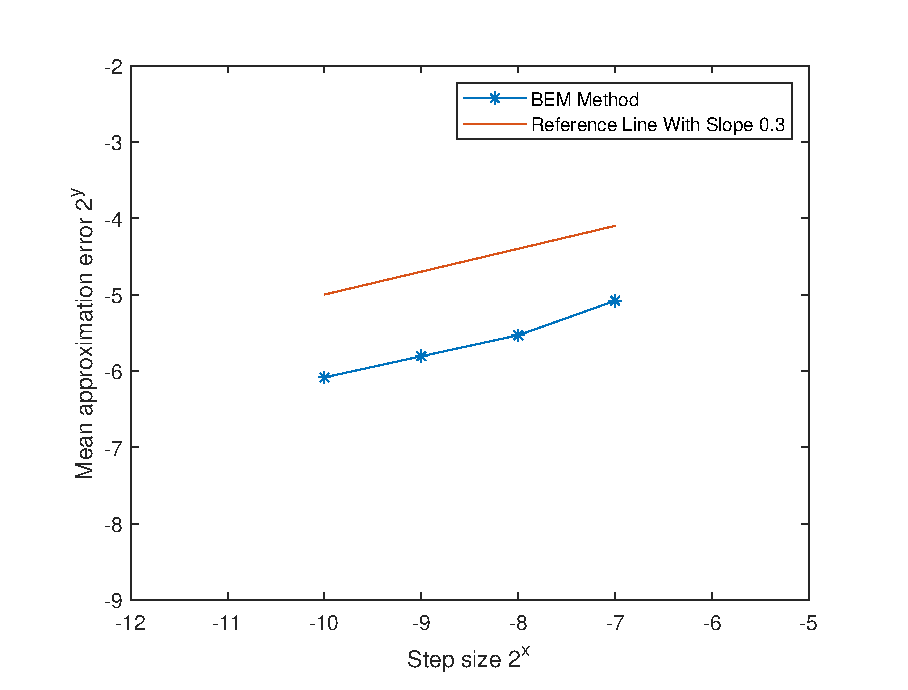
\includegraphics[width=0.45\linewidth]{BEMalpha=0.3.eps}
		\hfill
		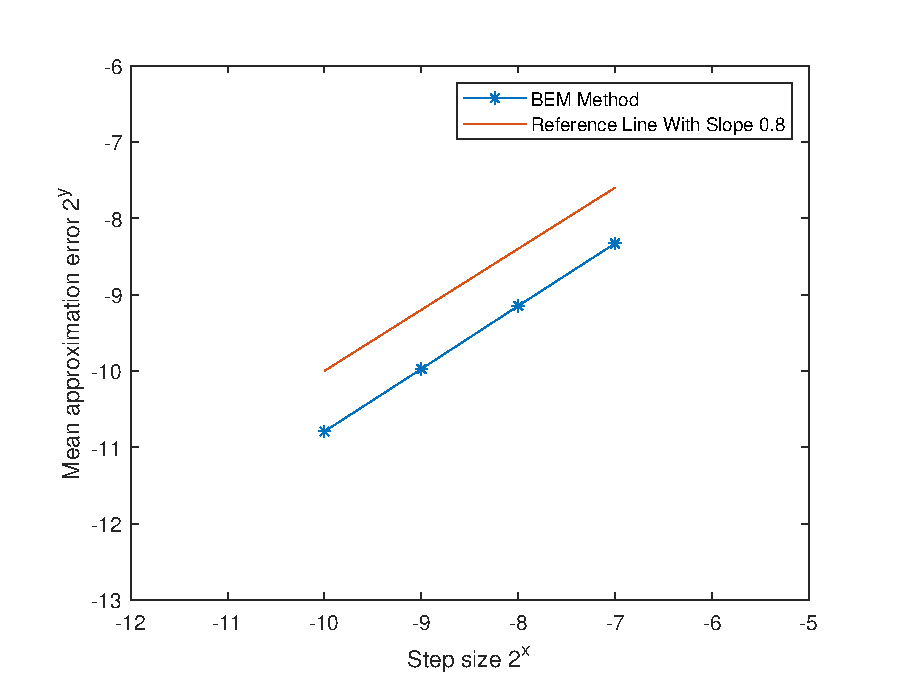
\includegraphics[width=0.45\linewidth]{BEMalpha=0.8.eps}
		\caption{时变CIR过程的BEM方法的$L_1$误差,左图是$\alpha=0.3$,右图是$\alpha=0.8$}
		\label{fig:image}
		\vspace{-2ex}
	\end{figure}
	
	\section{Present Job}
	我们想证明的是对于一个漂移项和扩散项都是非线性的时间变换SDE,将它进行Lamperti变换,变成漂移项是非线性,扩散项是常数的时间变换SDE,然后使用数值方法进行离散,得到与模拟代码一致的强收敛阶$\alpha$.截止当前的证明,我们已经证明了显式EM在$L^1$误差下的强收敛阶是$\alpha$,在证明$L^p$时,若使用之前的方法,得到的强收敛阶不仅与模拟的结果不一致,并且与p有关,强收敛阶与模拟代码不一致.证明的显示EM的强收敛阶,看起来对我们的预期没有什么意义,至少暂时我还没有找到对于原始非线性的漂移项扩散项经过Lamperti变换之后,得到的时变SDE漂移项满足全局Lipschitz,进而能够使用显示EM得到强收敛阶.下面对于变换后非线性的SDE,采用截断EM或者BEM,都会出现一个难以处理的东西,我们必须计算$L^2$误差,也就是$e^2$,这将导致不得不使用Gronwall不等式来处理这个式子,此时也会出现完全与p相关的收敛阶,那么我们可能需要换一个方法了.
	由于无法处理$L^2$误差,因此对于单调Lipschitz条件出现的平方项就无法使用。
	\textcolor{red}{至于Gronwall不等式,他在积分方面是几乎无法使用的,如果你选择先期望再Gronwall,会发现期望无法进入积分里面,这就导致了Gronwall条件不成立。然而如果先Gronwall再期望,则会发现离Gronwall条件相差十万八千里}
	% 开始附录部分
	\appendix
	\renewcommand{\appendixname}{附录} % 自定义附录标题
	
	\section{附录A}\label{appendix A}
	
	
	%%%%%%%%%%%%%%%%% 生成参考文献 %%%%%%%%%%%%%%%%%%%%%
	
	%\nocite{*}  % 可以暂时显示全部参考文献
	\bibliographystyle{plain}
	\bibliography{reference}
	
	
	
	
\end{document}

